% One continuous worksheet grid. The black dashed lines are the three given axes.
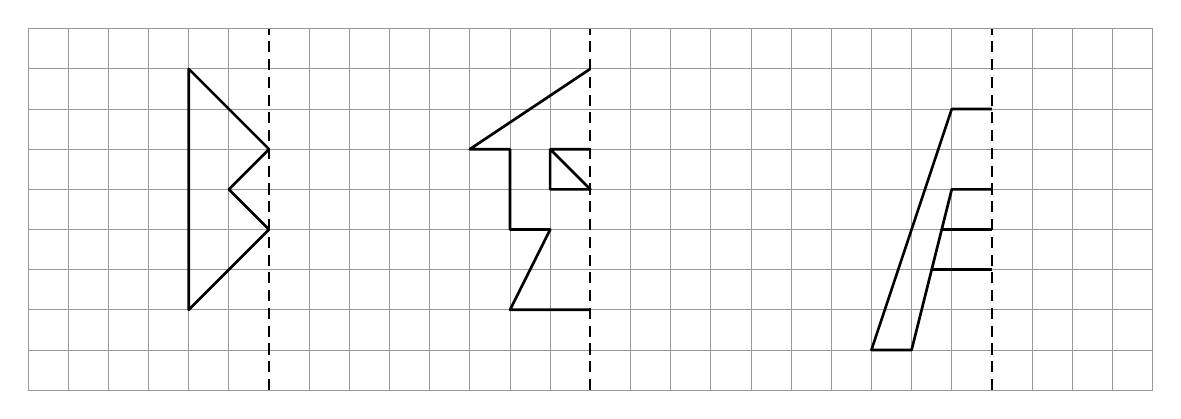
\begin{tikzpicture}[x=.51cm,y=.51cm,line cap=butt,line join=round]
  \foreach \x in {0,...,28}{
    \ifnum\x=6\else\ifnum\x=14\else\ifnum\x=24\else
      \draw[black!40,line width=.32bp] (\x,0)--(\x,9);
    \fi\fi\fi}
  \foreach \y in {0,...,9}
    \draw[black!40,line width=.32bp] (0,\y)--(28,\y);
  \foreach \x in {6,14,24}
    \draw[line width=.75bp,dash pattern=on 4bp off 2.4bp] (\x,0)--(\x,9);
  \begin{scope}[line width=.95bp]
    \draw (4,8)--(6,6)--(5,5)--(6,4)--(4,2)--cycle;
    % Second half-figure on the shared grid, with its original interior strokes.
\draw (14,8)--(11,6)--(12,6)--(12,4)--(13,4)--(12,2)--(14,2);
\draw (14,6)--(13,6)--(13,5)--(14,5)--(13,6);

    % Third half-figure on the shared grid.
\draw (24,7)--(23,7)--(21,1)--(22,1)--(23,5)--(24,5);
\draw (22.75,4)--(24,4) (22.5,3)--(24,3);

  \end{scope}
\end{tikzpicture}
